\section{CBS Measurement Details} \label{sec:cbs-measurement-details}

Our empirical method for measuring the CBS \Cref{sec:our-method} is, in principle, sensitive to the choice of checkpoints and batch size multipliers.
We therefore document the checkpoints and multipliers we used here.

\paragraph{OLMo 1B.}
When measuring the OLMo 1B CBS with branching, we set the base batch size to 1024 and the base learning rate to $0.0004 \cdot \sqrt{2}$, reflecting the default batch size of 512 and learning rate of 0.0004 in the OLMo codebase under a square-root scaling rule \citep{malladi2022sdes}.
We then chose the following checkpoints and multipliers $k$:
\begin{enumerate}
    \item Step 0: $k$ ranging over 0.0625, 0.125, 0.25.
    \item Steps 10K, 20K, $\ldots$, 50K: $k$ ranging over 0.5, 1, $\ldots$, 5.
    \item Steps 100K, 150K, $\dots$, 450K: $k$ ranging over 1, 2, $\ldots$, 8.
\end{enumerate}
\Cref{fig:all-losses-1b} shows loss vs.~batch size plots for all checkpoints of OLMo 1B.

\paragraph{OLMo 7B.} We set the base batch size to 1024 and the base learning rate to $0.0003$, as specified in the OLMo codebase.
We then chose the following checkpoints and multipliers $k$:
\begin{enumerate}
    \item Step 0: $k$ ranging over 0.0625, 0.125, 0.25.
    \item Steps 1K, 2K, 3K: $k$ ranging over 0.25, 0.5, 1, 2, 3, 4.
    \item Steps 10K, 20K, 30K: $k$ ranging over 1, 2, 3, 4, 5.
    \item Steps 72K, 150K, 200K, 239K, 300K, 350K, 400K, 477K: $k$ ranging over 1, 2, 3, 4, 5, 6, 7, 8.
\end{enumerate}
\Cref{fig:all-losses-7b} shows loss vs.~batch size plots for all checkpoints of OLMo 7B.
These checkpoints were chosen manually as we developed this project.
Over the course of our experimentation, we launched many additional runs beyond the ones discussed above.
Since the choice of $k$ can influence the conclusions of our method, we filtered down the included runs to make the choice of $k$ systematic.

1B runs were launched on a single node of H100 GPUs, and 7B runs were launched on 8 nodes.

\begin{figure}
    \centering
    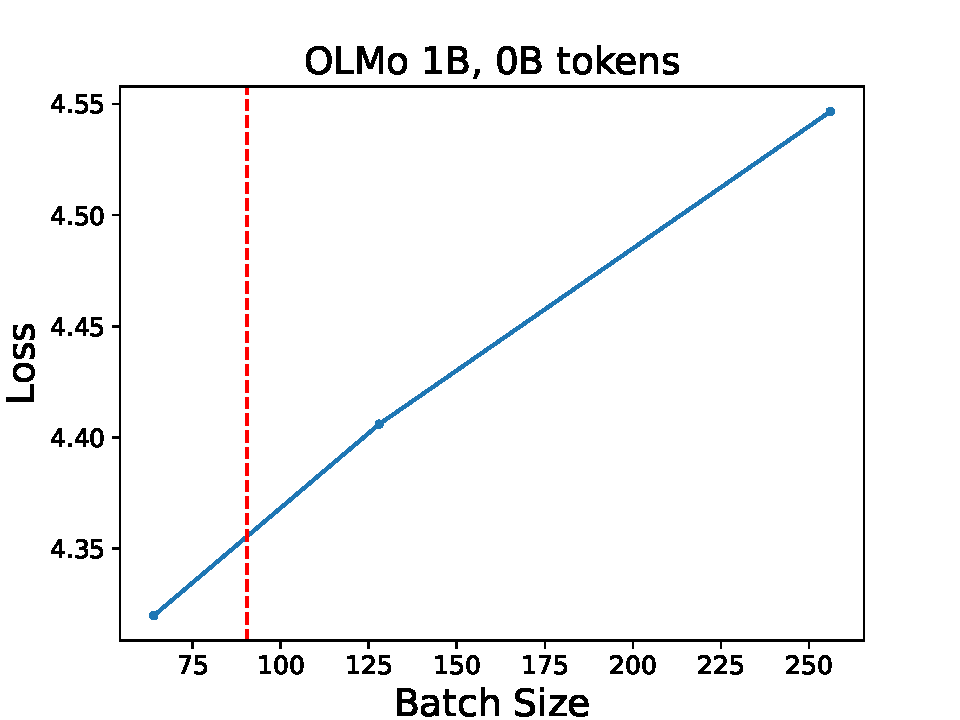
\includegraphics[width=0.32\linewidth]{figures/measure-cbs/peteish1-fixlr/from0.pdf}
    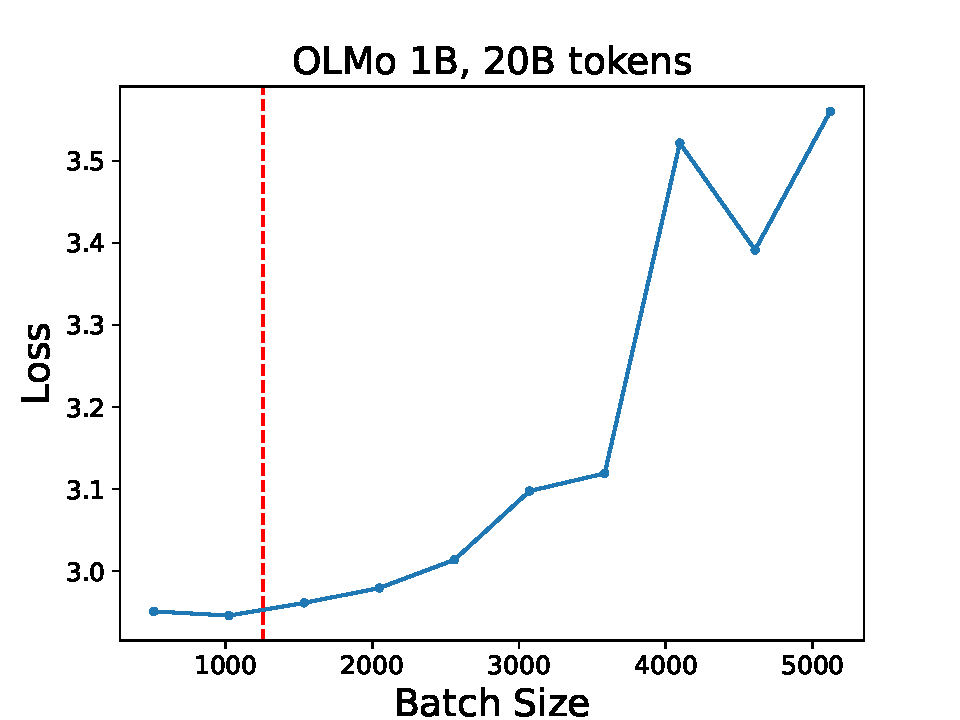
\includegraphics[width=0.32\linewidth]{figures/measure-cbs/peteish1-fixlr/from10000.pdf}
    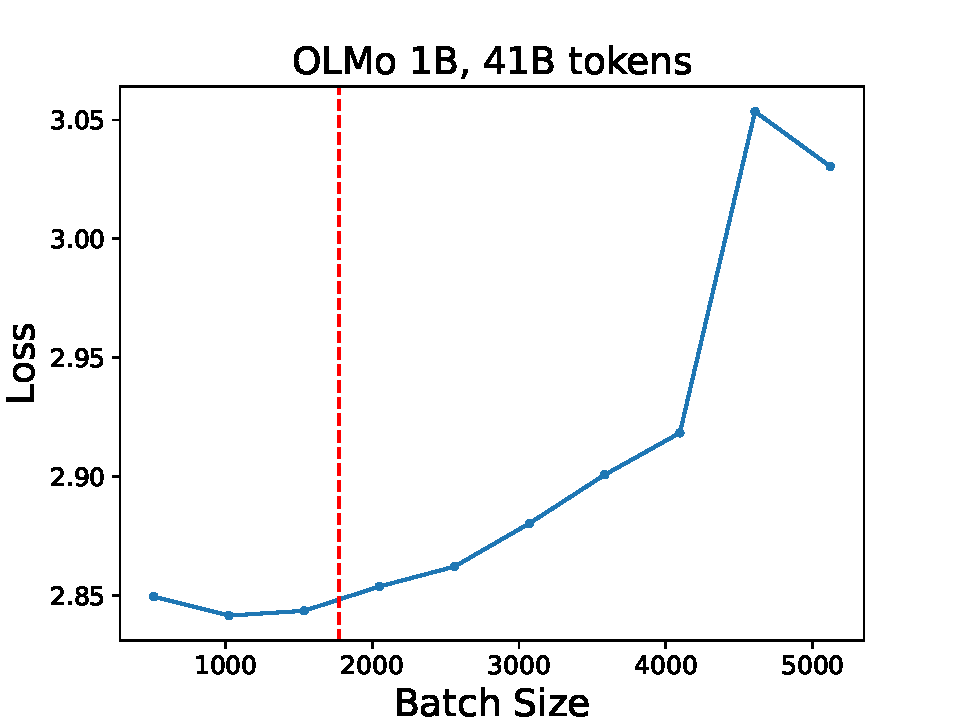
\includegraphics[width=0.32\linewidth]{figures/measure-cbs/peteish1-fixlr/from20000.pdf}
    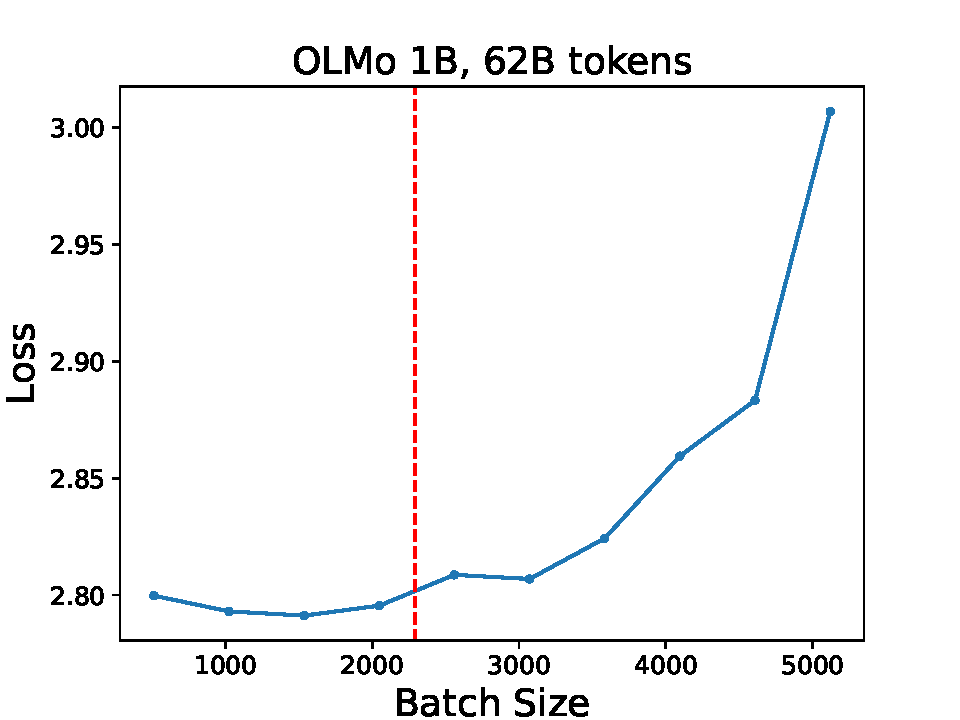
\includegraphics[width=0.32\linewidth]{figures/measure-cbs/peteish1-fixlr/from30000.pdf}
    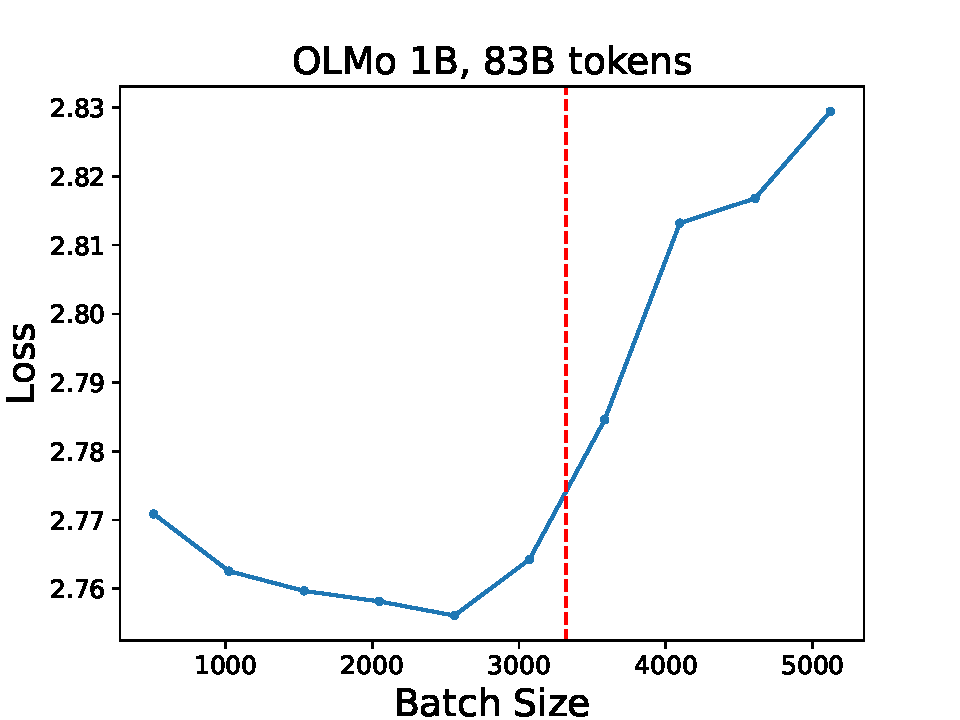
\includegraphics[width=0.32\linewidth]{figures/measure-cbs/peteish1-fixlr/from40000.pdf}
    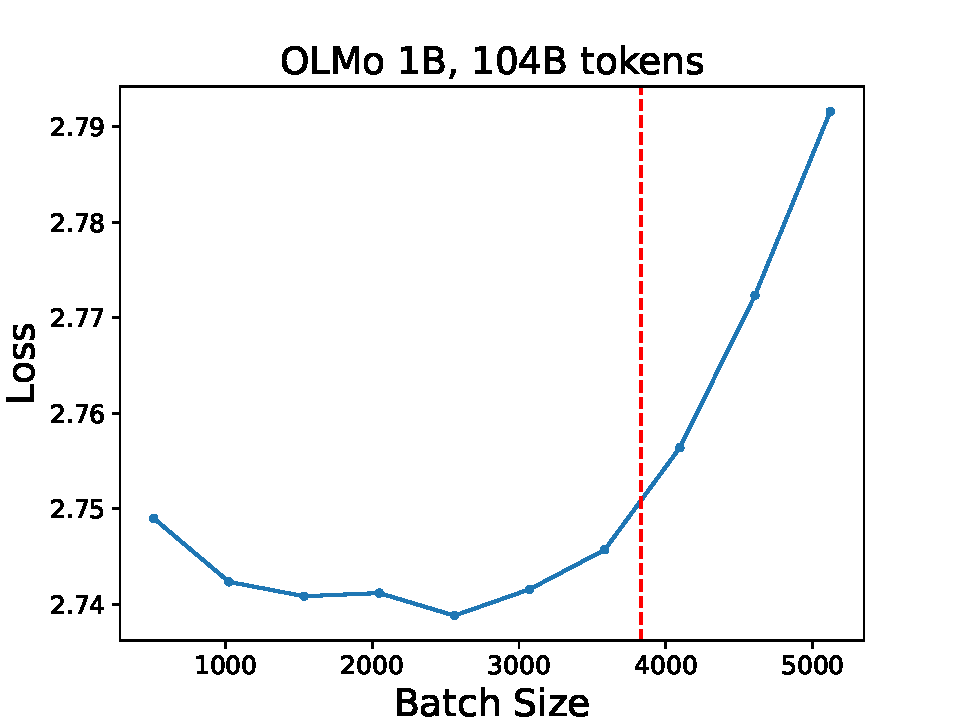
\includegraphics[width=0.32\linewidth]{figures/measure-cbs/peteish1-fixlr/from50000.pdf}
    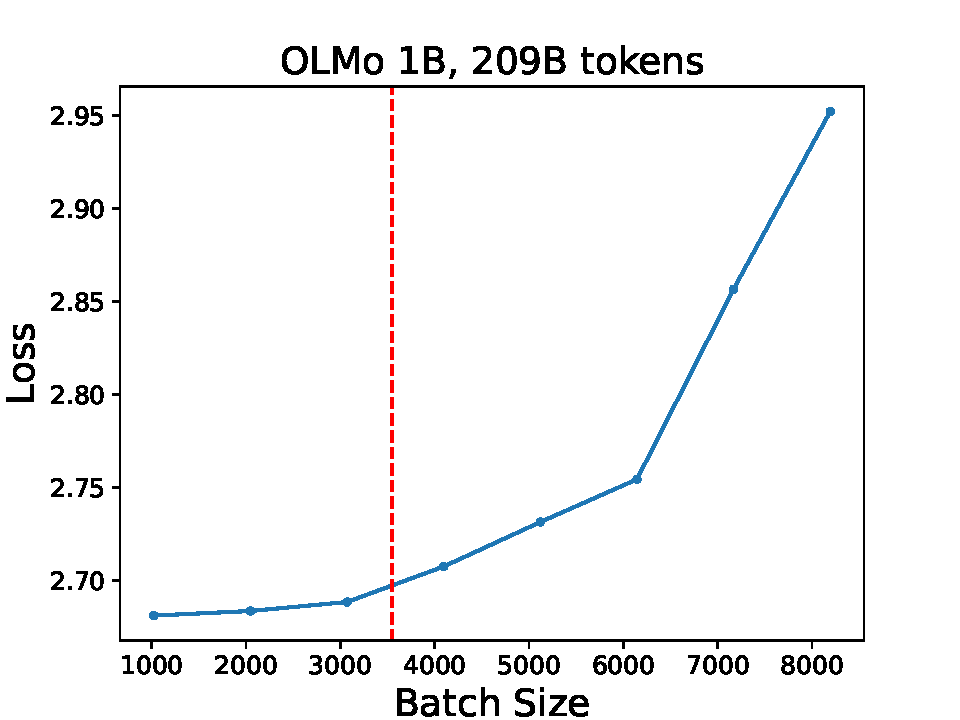
\includegraphics[width=0.32\linewidth]{figures/measure-cbs/peteish1-fixlr/from100000.pdf}
    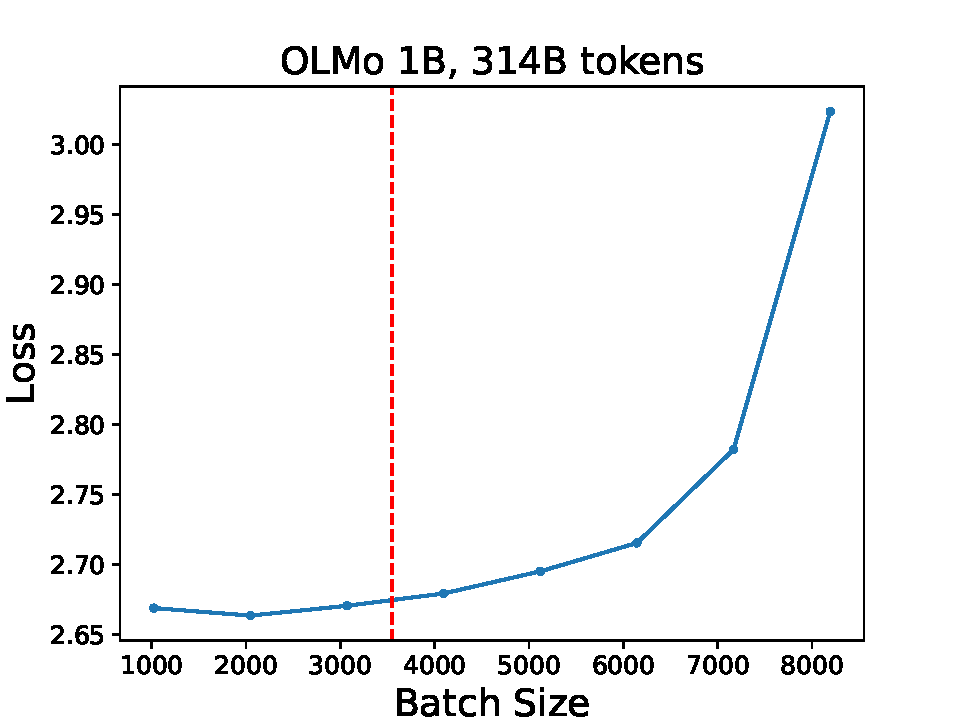
\includegraphics[width=0.32\linewidth]{figures/measure-cbs/peteish1-fixlr/from150000.pdf}
    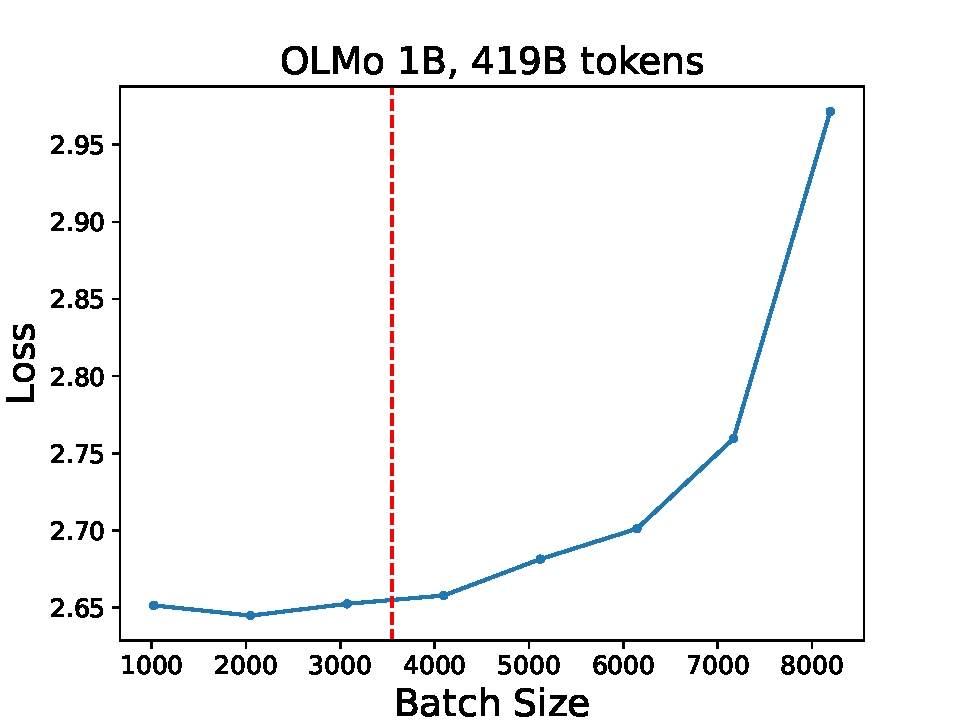
\includegraphics[width=0.32\linewidth]{figures/measure-cbs/peteish1-fixlr/from200000.pdf}
    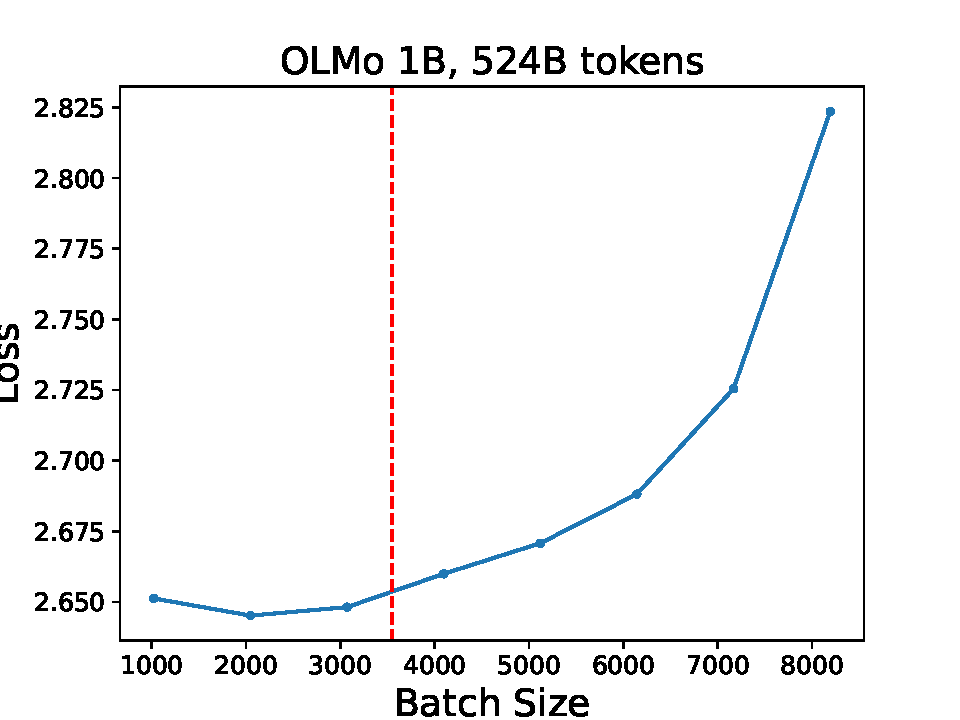
\includegraphics[width=0.32\linewidth]{figures/measure-cbs/peteish1-fixlr/from250000.pdf}
    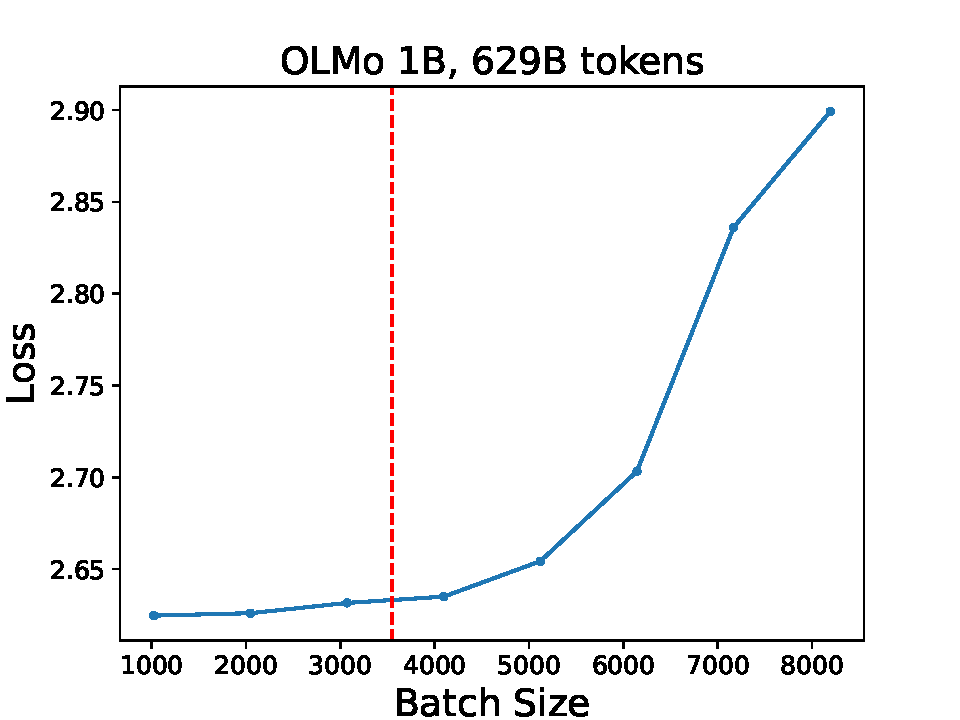
\includegraphics[width=0.32\linewidth]{figures/measure-cbs/peteish1-fixlr/from300000.pdf}
    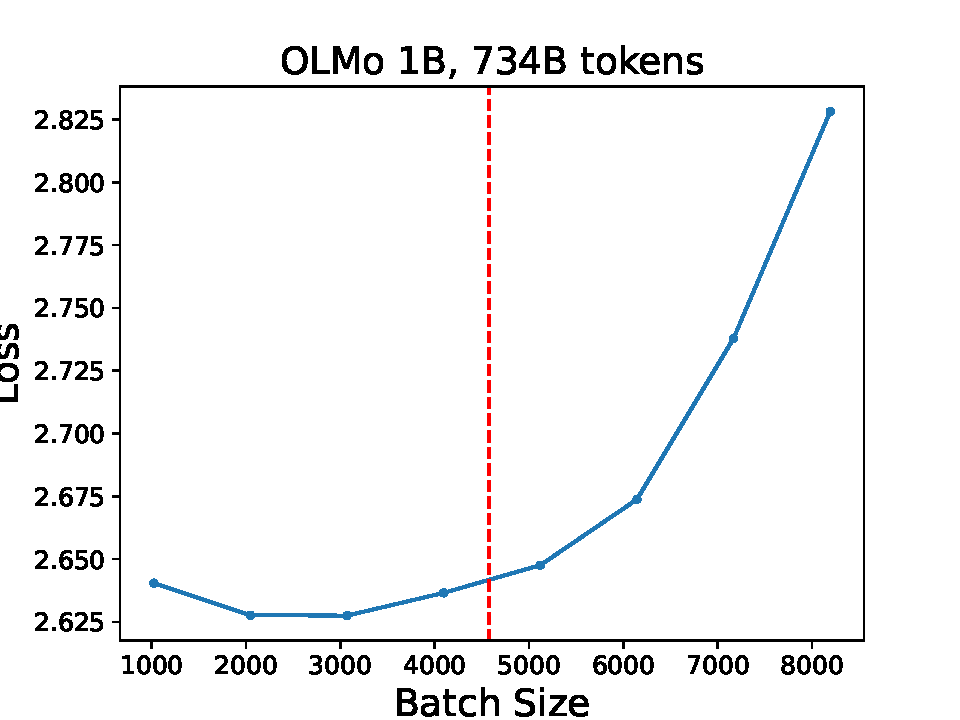
\includegraphics[width=0.32\linewidth]{figures/measure-cbs/peteish1-fixlr/from350000.pdf}
    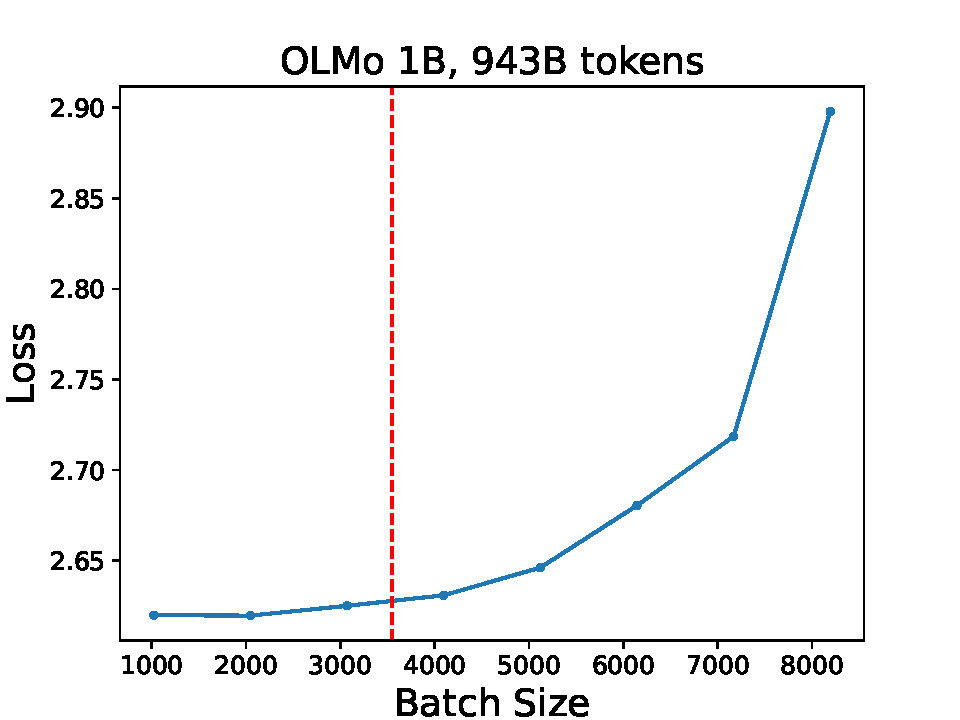
\includegraphics[width=0.32\linewidth]{figures/measure-cbs/peteish1-fixlr/from450000.pdf}
    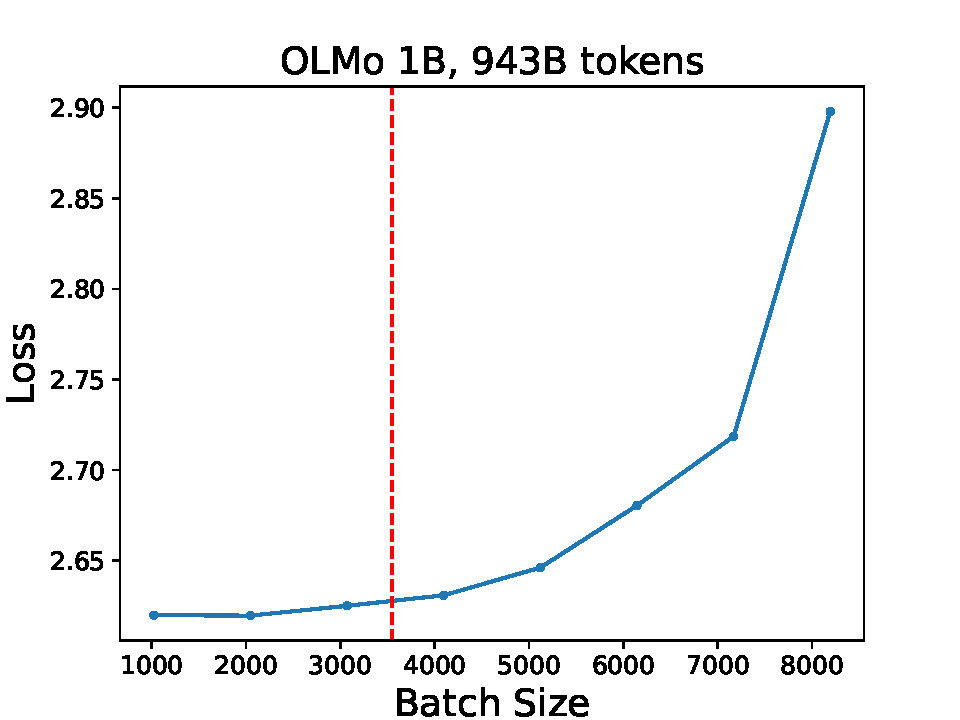
\includegraphics[width=0.32\linewidth]{figures/measure-cbs/peteish1-fixlr/from450000.pdf}
    \caption{All loss vs. batch size plots for OLMo 1B. Overall, the red line moves to the right over time, showing that the CBS increases.}
    \label{fig:all-losses-1b}
\end{figure}

\begin{figure}
    \centering
    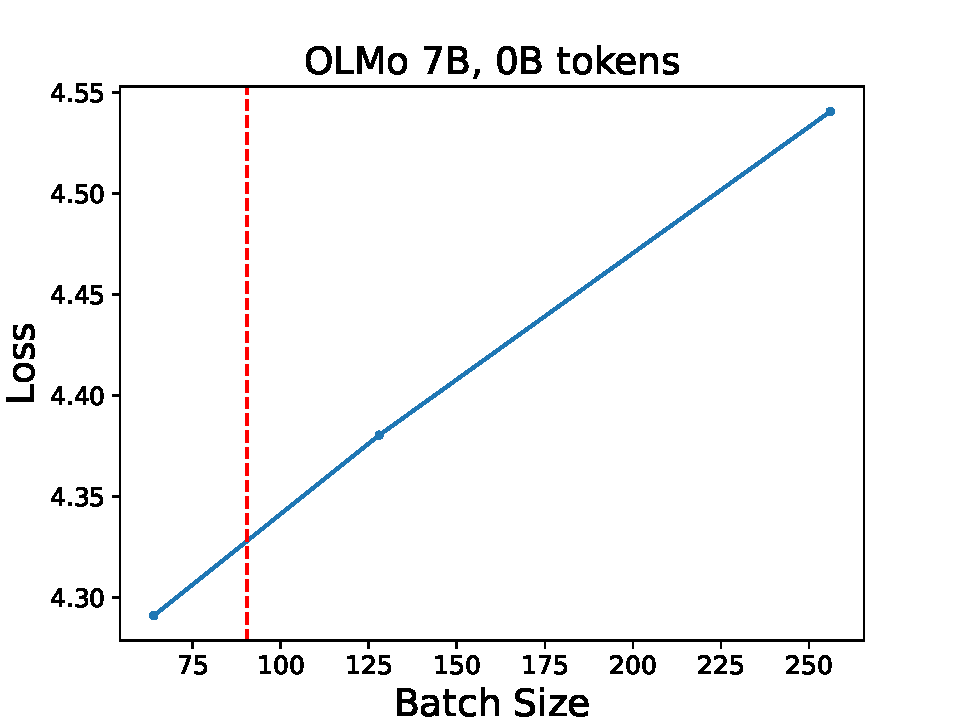
\includegraphics[width=0.32\linewidth]{figures/measure-cbs/peteish7/from0.pdf}
    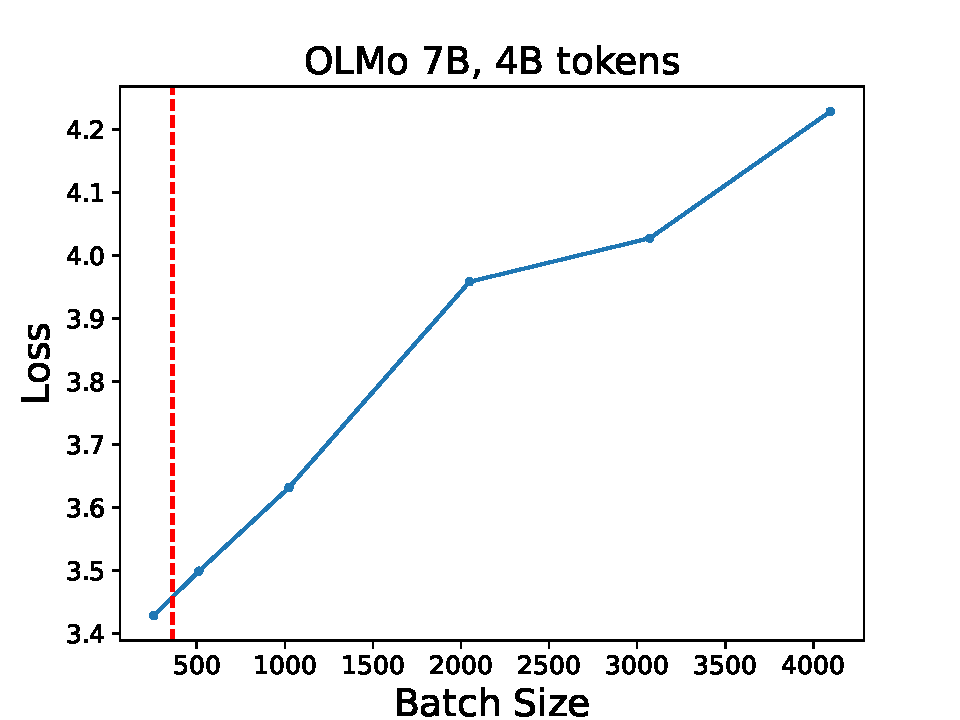
\includegraphics[width=0.32\linewidth]{figures/measure-cbs/peteish7/from1000.pdf}
    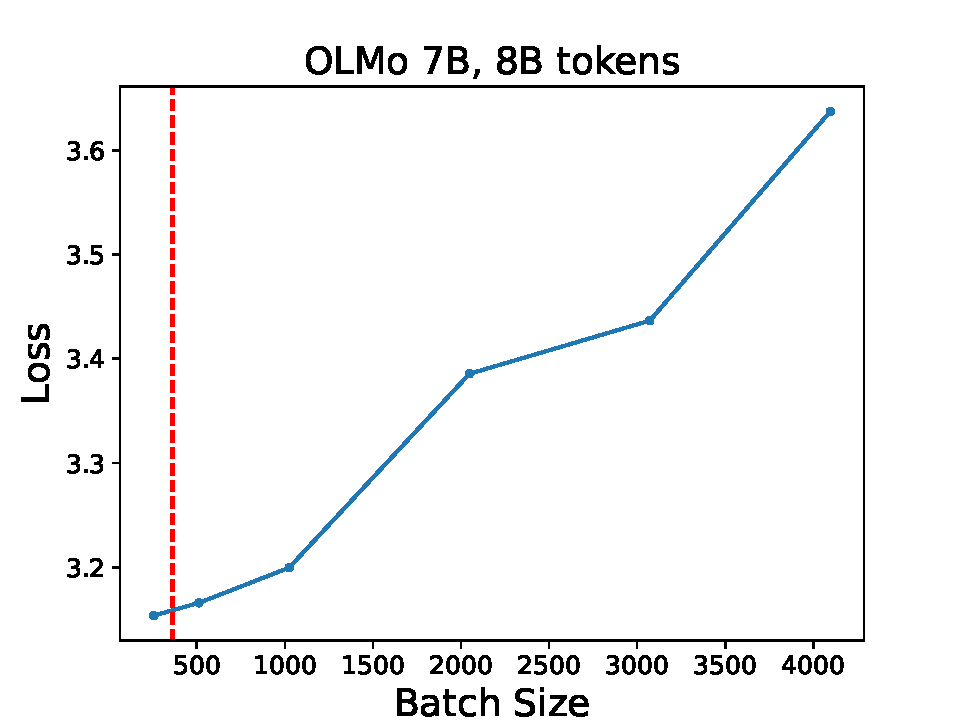
\includegraphics[width=0.32\linewidth]{figures/measure-cbs/peteish7/from2000.pdf}
    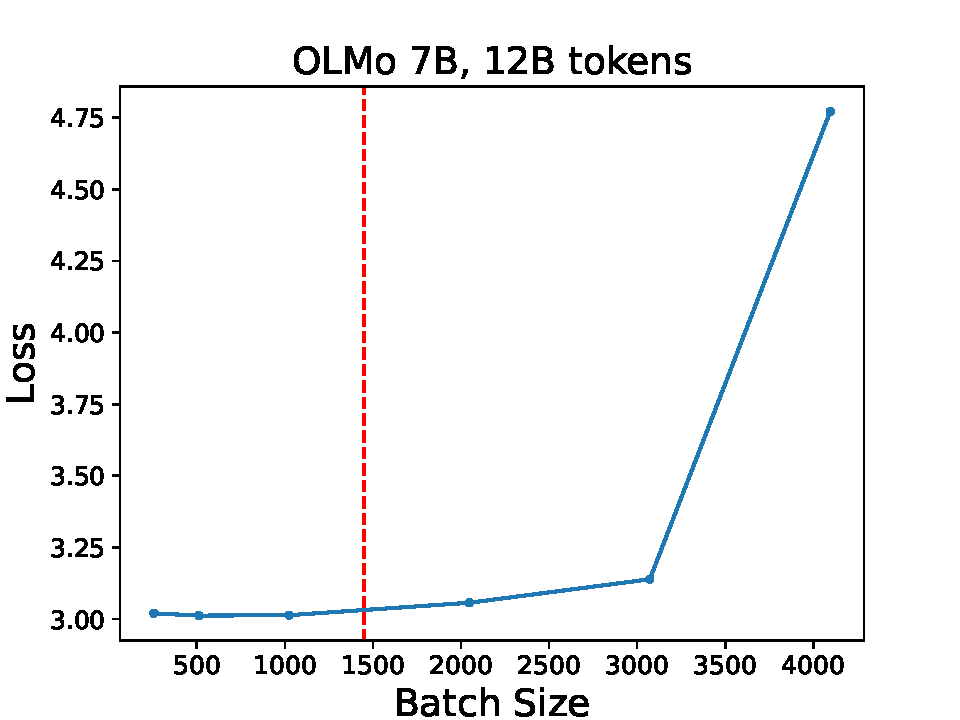
\includegraphics[width=0.32\linewidth]{figures/measure-cbs/peteish7/from3000.pdf}
    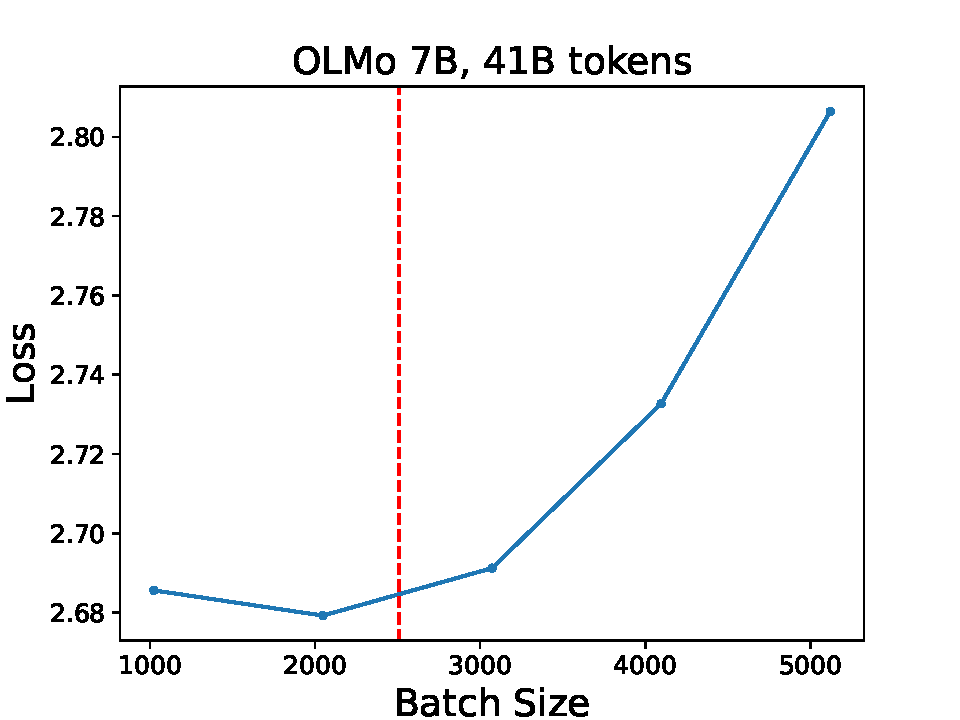
\includegraphics[width=0.32\linewidth]{figures/measure-cbs/peteish7/from10000.pdf}
    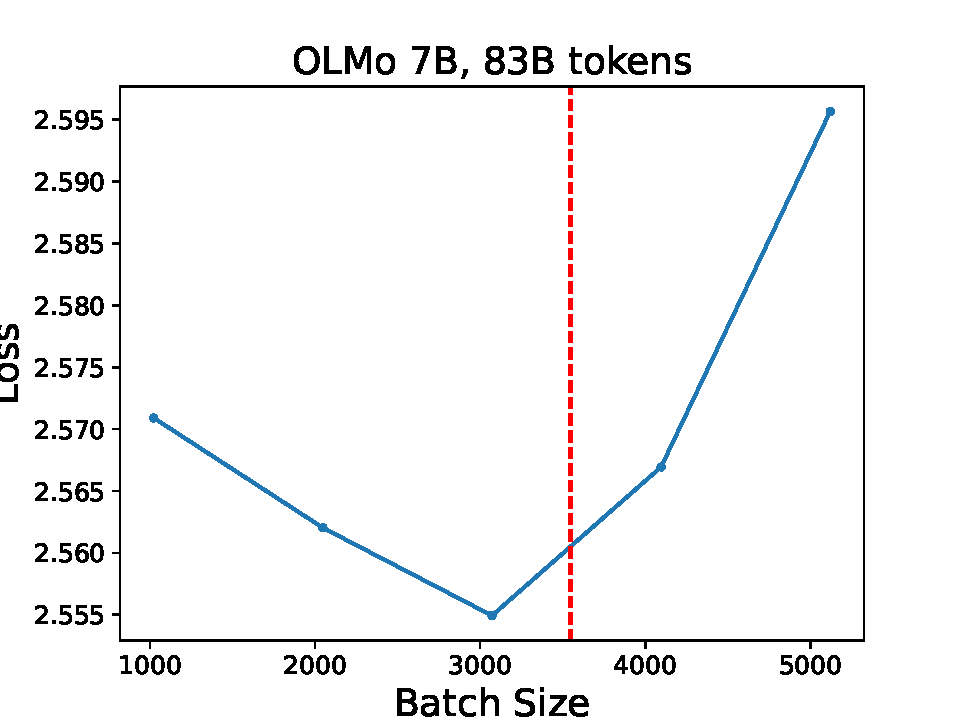
\includegraphics[width=0.32\linewidth]{figures/measure-cbs/peteish7/from20000.pdf}
    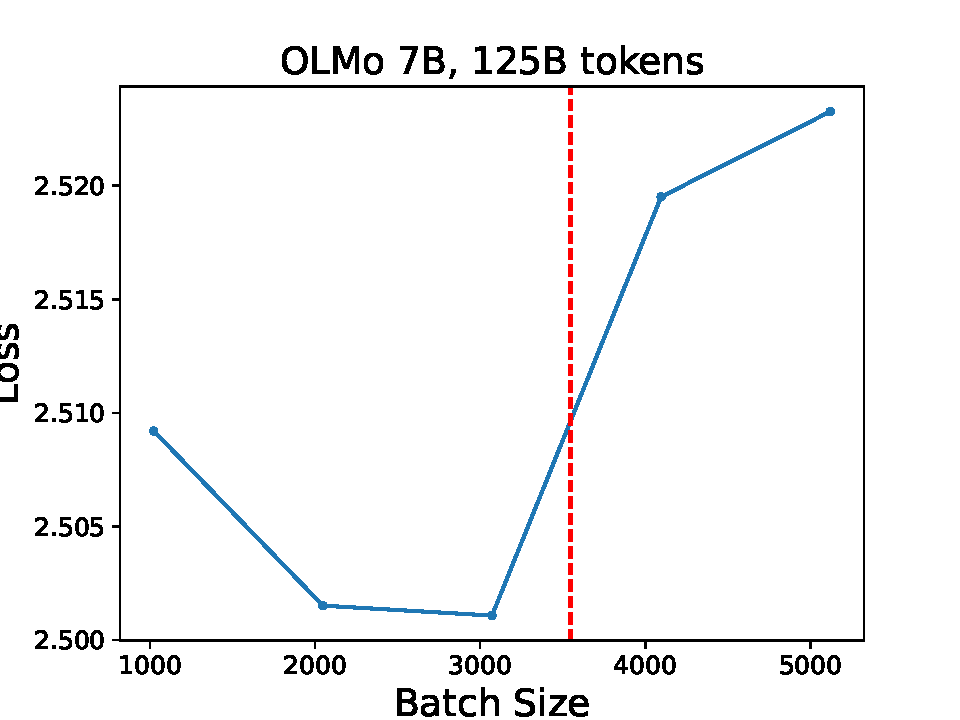
\includegraphics[width=0.32\linewidth]{figures/measure-cbs/peteish7/from30000.pdf}
    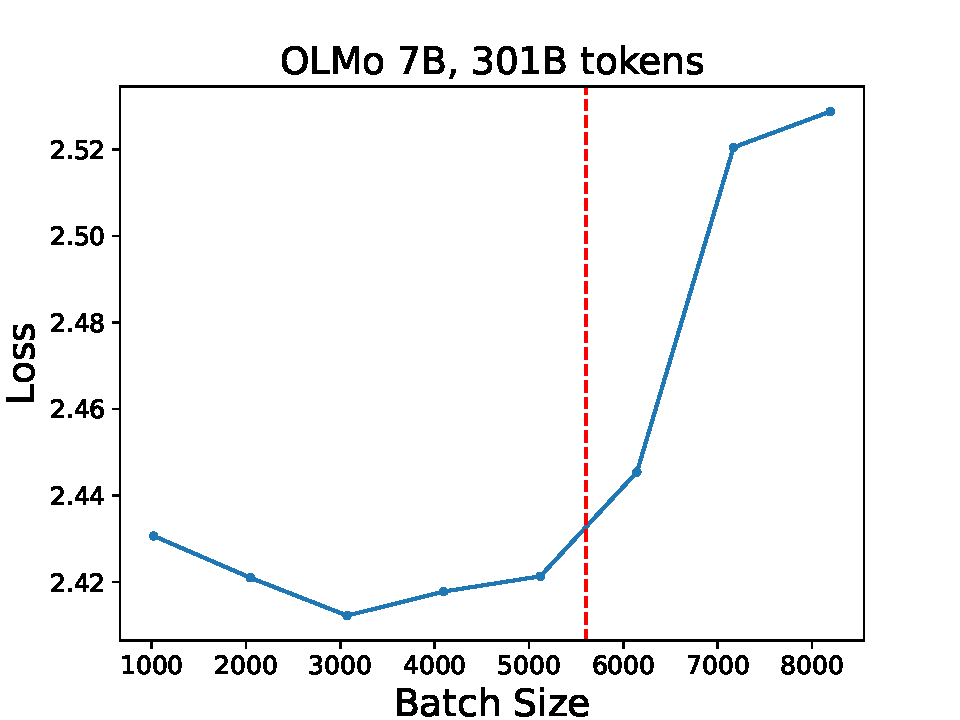
\includegraphics[width=0.32\linewidth]{figures/measure-cbs/peteish7/from72000.pdf}
    % \includegraphics[width=0.32\linewidth]{figures/measure-cbs/peteish7/from100000.pdf}
    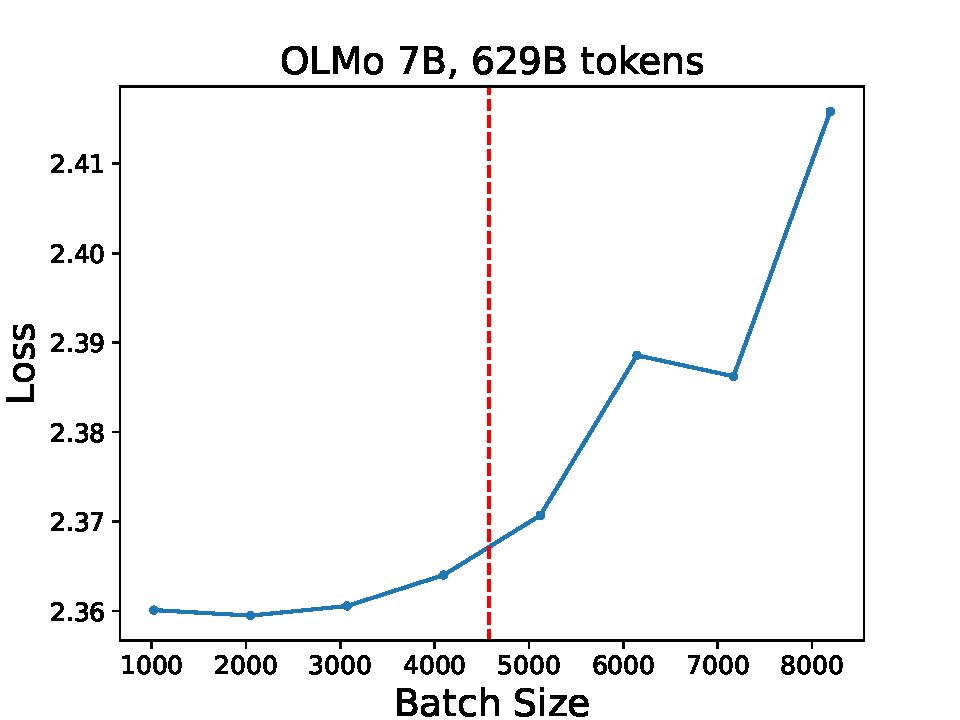
\includegraphics[width=0.32\linewidth]{figures/measure-cbs/peteish7/from150000.pdf}
    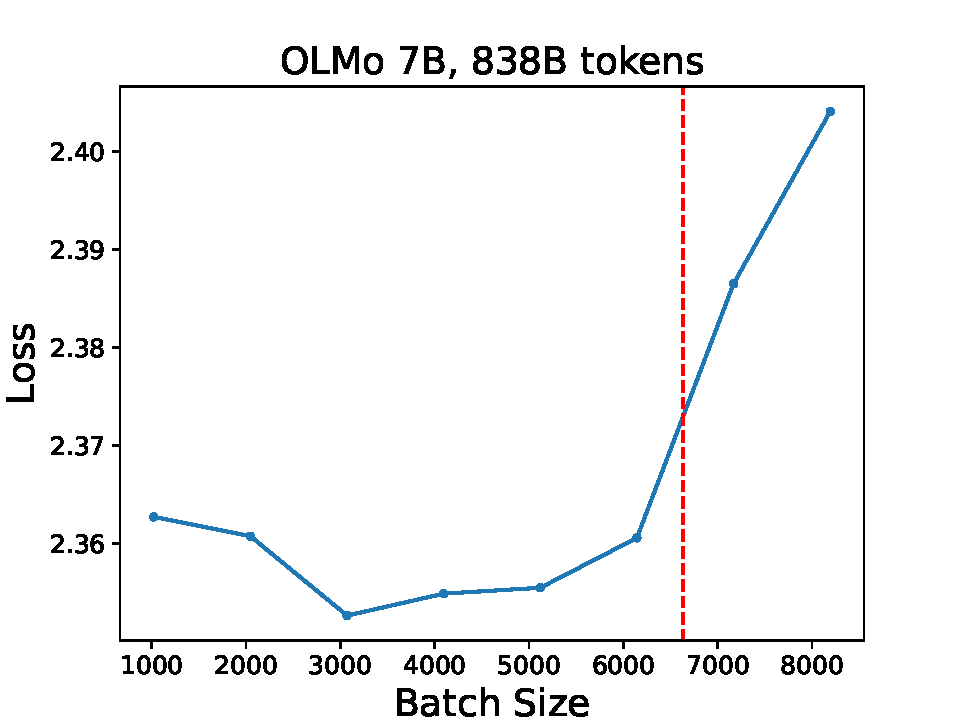
\includegraphics[width=0.32\linewidth]{figures/measure-cbs/peteish7/from200000.pdf}
    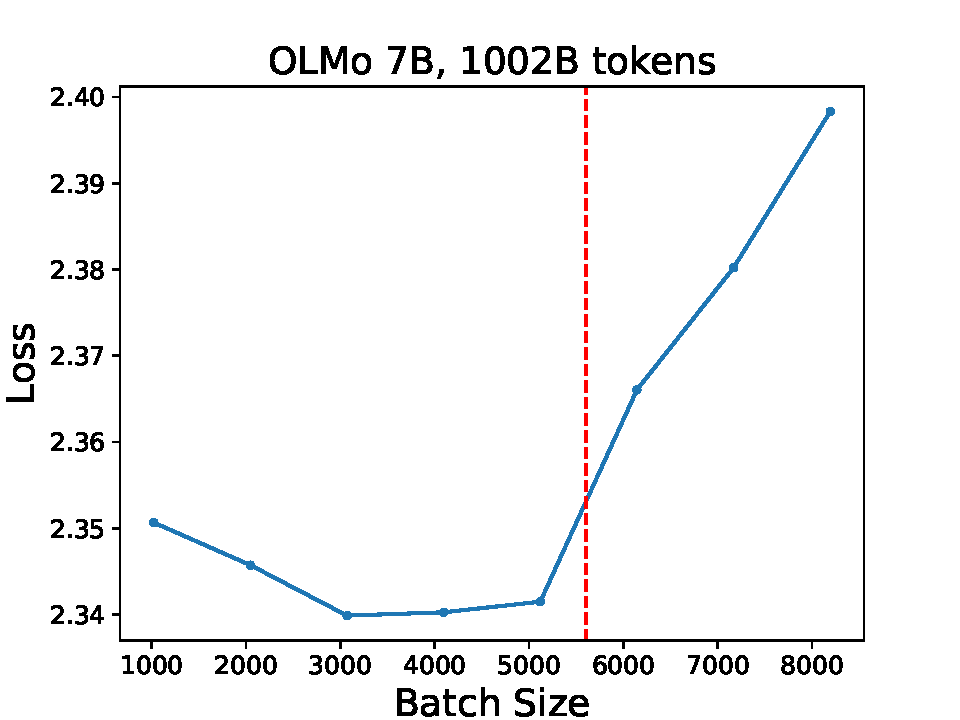
\includegraphics[width=0.32\linewidth]{figures/measure-cbs/peteish7/from239000.pdf}
    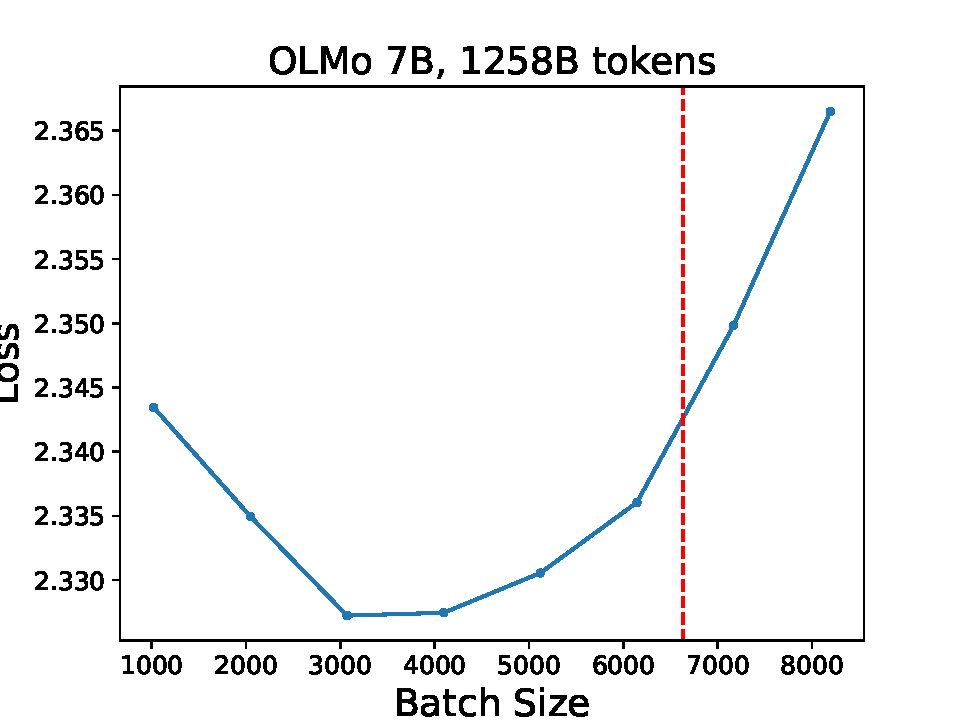
\includegraphics[width=0.32\linewidth]{figures/measure-cbs/peteish7/from300000.pdf}
    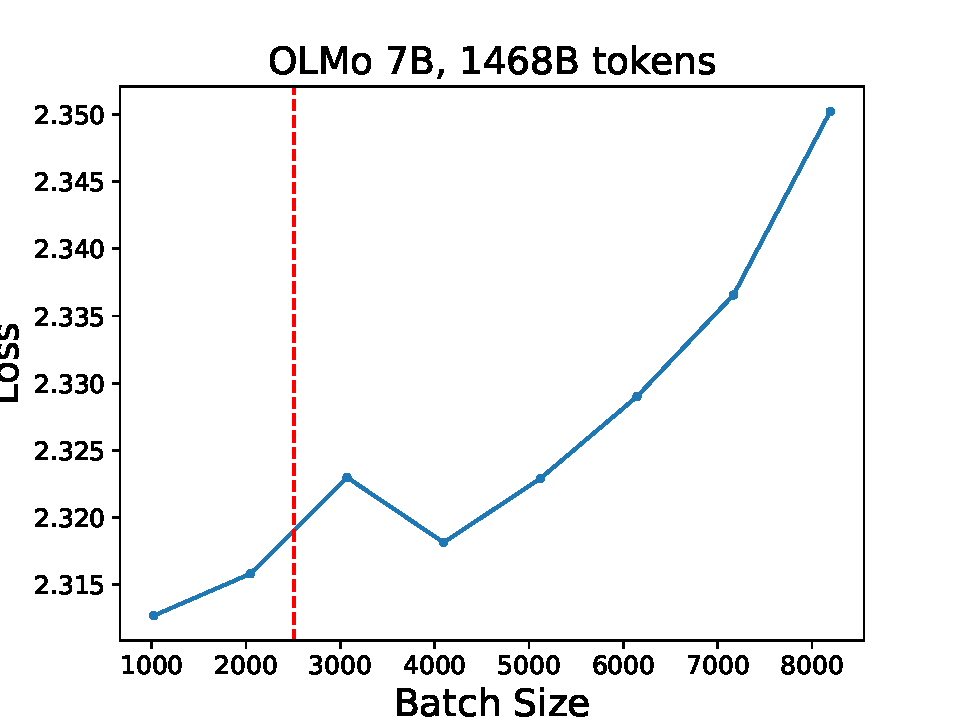
\includegraphics[width=0.32\linewidth]{figures/measure-cbs/peteish7/from350000.pdf}
    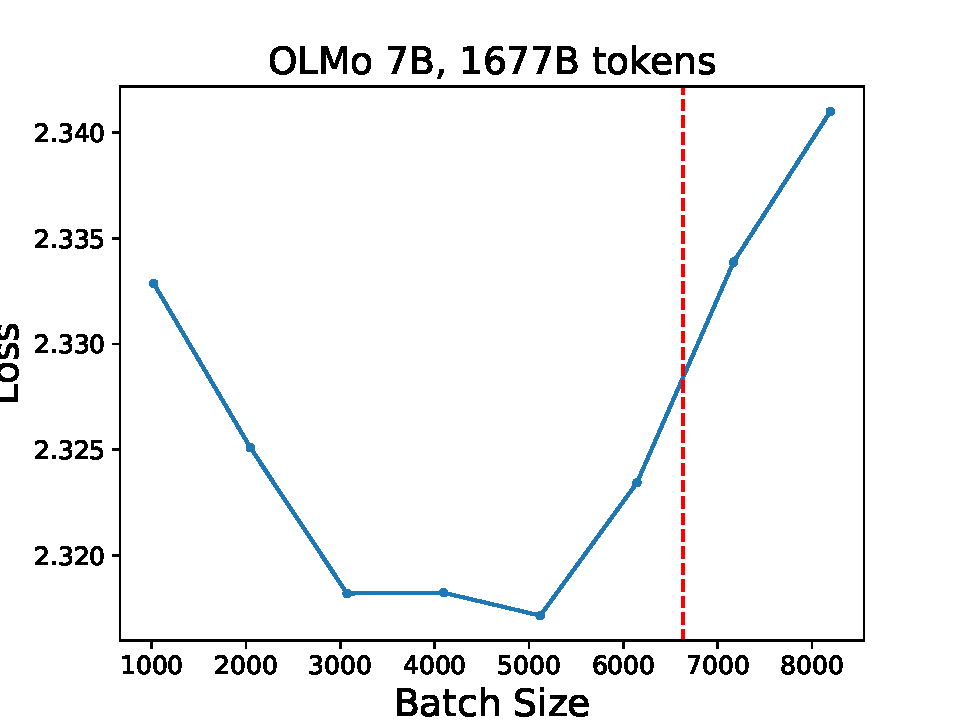
\includegraphics[width=0.32\linewidth]{figures/measure-cbs/peteish7/from400000.pdf}
    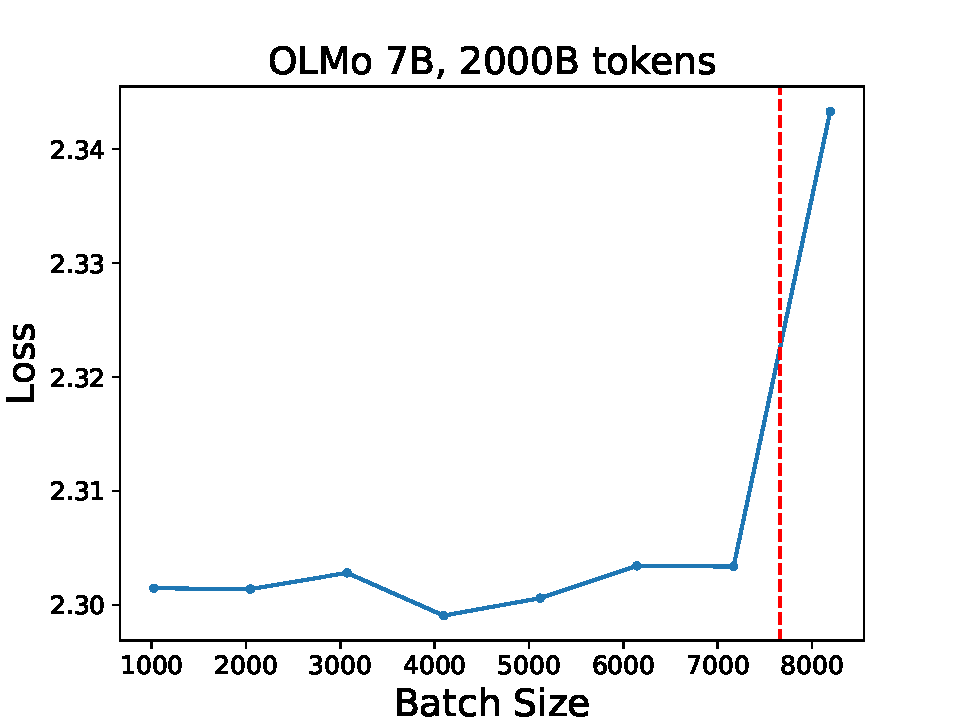
\includegraphics[width=0.32\linewidth]{figures/measure-cbs/peteish7/from477000.pdf}
    \label{fig:all-losses-7b}
\end{figure}

\section{Noise Scale Measurement Details} \label{app:noise-scale}

We use the gradient noise scale estimator proposed by \citet[Appendix A]{mccandlish2018empirical} to estimate the gradient noise scale.
The method estimates the gradient noise scale using gradient norms at two different batch sizes $\Bbig$ and $\Bsmall$ according to:
\begin{align*}
    \mathcal B_\mathrm{simple} &\approx \frac{\mathcal S}{\norm{\mathcal G}^2} , \textrm{where} \\
    \mathcal S &= \frac{\nGsmall - \nGbig}{1/\Bsmall - 1/\Bbig} \\
    \norm{\mathcal G}^2 &= \frac{\Bbig \nGbig - \Bsmall \nGsmall}{\Bbig - \Bsmall} . \\
\end{align*}
We use large batch size $\Bbig = 64$ and small batch size $\Bsmall = 1$.

It holds that $\mathbb{E} \left[ \mathcal S \right] = \mathrm{tr}(\Sigma)$ and $\mathbb{E} \left[ \norm{\mathcal G}^2 \right] = \norm{G}^2$. We thus average $\mathcal S$ and $\norm{\mathcal G}^2$ over 4096 batches reduce variance and then return their ratio as our estimate of the noise scale $\mathcal B_\mathrm{simple}$, using offline (i.e., unseen) data in each batch.

We estimate a confidence interval for $\mathcal B_\mathrm{simple}$ in two steps. First, we estimate 95\% confidence intervals for $\mathcal S$ and $\norm{\mathcal G}^2$, assuming the data are exponentially\footnote{For the exponential distribution, we use approximate confidence interval under ``Confidence Intervals'' here: \url{https://en.wikipedia.org/wiki/Exponential_distribution}.} and normally distributed, respectfully, based on manual inspection of their distributions (cf.~\Cref{fig:distributions}).
We denote these intervals $[a_{\mathcal S}, b_{\mathcal S}]$ and $[a_{\norm{\mathcal G}^2}, b_{\norm{\mathcal G}^2}]$, respectively.
We then define the confidence interval for $\mathcal B_\mathrm{simple}$ as follows:
\begin{equation*}
    \left[ \frac{a_{\mathcal S}}{b_{\norm{\mathcal G}^2}}, \frac{b_{\mathcal S}}{a_{\norm{\mathcal G}^2}} \right] .
\end{equation*}

If our estimates for $\mathcal S$ or $\norm{\mathcal G}^2$ (or their lower or upper bounds) come out negative, we consider them to be 0.

The checkpoints considered for OLMo 1B are steps 0, 10K, 20K, 40K, $\ldots$, 100K, 200K, $\ldots$ 400K.
For OLMo 7B, we use checkpoints at steps 0, 10K, $\ldots$, 40K, 60K, 70K, $\ldots$, 100K, 200K, $\ldots$ 400K.
The noise scale experiment for each checkpoint (for both the 1B and 7B models) was launched on a single GPU.

\begin{figure}
    \centering
    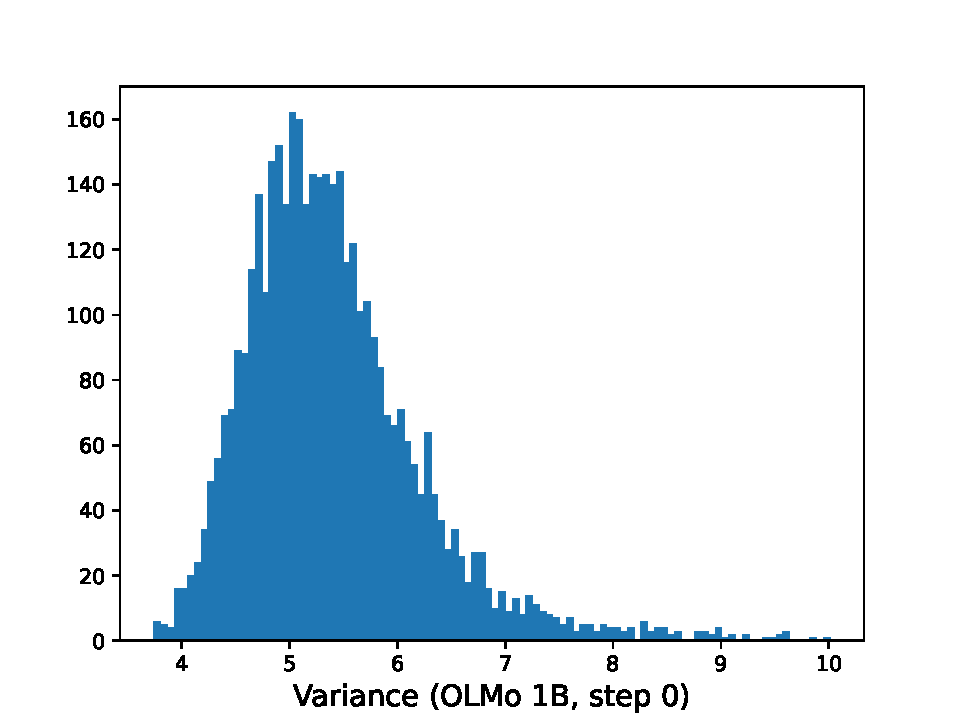
\includegraphics[width=0.48\linewidth]{figures/noise-scale/peteish1/variance.pdf}
    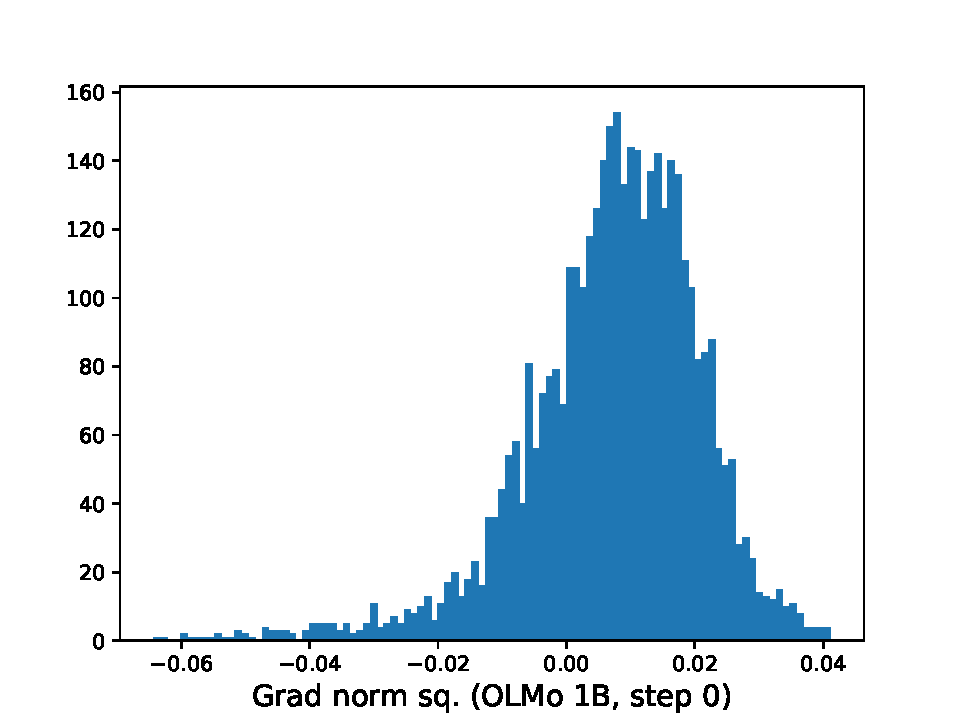
\includegraphics[width=0.48\linewidth]{figures/noise-scale/peteish1/grad-norm.pdf}
    \caption{Representative histograms for $\mathcal S$ and $\norm{\mathcal G}^2$, showing data from the 1st to 99th percentiles. The distribution for $\mathcal S$ is positive, leading us to use an exponential distribution, while the fact that some samples of $\norm{\mathcal G}^2$ are negative motivates a normal distribution.}
    \label{fig:distributions}
\end{figure}

\section{License Information} \label{sec:other-details}

The OLMo models \citep{groeneveld-etal-2024-olmo,olmo20252olmo2furious} and pretraining code, which we use, are released under Apache-2.0 license.
C4 \citep{C4} is released under ODC-BY license.
The Pile \citep{Pile} is released under MIT license.

\section{Deriving CBS Scaling Laws: An Attempt} \label{sec:scaling-laws}

In this section, we explore whether our empirical fits for the critical batch size over training can be used to derive scaling laws for aggregate critical batch size that have been derived in prior work. These scaling laws assume we want to use a fixed batch size $B$ over training, and then train many different models to the same target loss. They then measure the critical $B^*$ up to which increases in batch size do not diminish token efficiency. The standard finding from such work is that CBS grows $\propto \sqrt{T}$, where $T$ is the total training budget in tokens. This is consistent with our finding that CBS increases over the course of training---moreover, we now seek to analyze whether this scaling law can be derived from our empirical measurements of local CBS. If so, this would provide converging evidence and a simpler method for fitting CBS scaling laws that only requires training a single model.

To begin, we assume that the goal of picking a fixed batch size $B$ is to minimize the L2 distance to the local CBS over the course of training.
It is not obvious that minimizing L2 distance is the right way to pick the fixed CBS: for instance, we might want to weight training at a batch size \emph{above} the local CBS more negatively than training below it.
Regardless, we will proceed for now under the assumption that this is the right perspective.
We also make the weaker assumption that $f(t) = 0$, in line with our empirical findings (\Cref{sec:our-method}).
It follows that the best batch size to train at (i.e., fixed CBS) is simply the average local CBS over training:

\begin{restatable}{proposition}{residuals} \label{thm:residuals}
    Let $f(t)$ be integrable with $f(0) = 0$ and define
    \begin{equation*}
        R_2 = \sqrt{\int_0^T \left( B - f(t) \right)^2 \mathrm{d}t} .
    \end{equation*}
    Then $R_2$ is minimized by $B^* = \frac{1}{T} \int_0^T f(t) \mathrm{d} t$.
\end{restatable}

\begin{proof}
    We can first simplify the expression for $(R_2)^2$:
    \begin{align*}
        (R_2)^2
        &= \int_0^T \left( B - f(t) \right)^2 \mathrm{d}t \\
        &= \int_0^T \left( B^2 - 2Bf(t) + f(t)^2 \right) \mathrm{d}t \\
        &= B^2T - \int_0^T \left( 2Bf(t) - f(t)^2 \right) \mathrm{d}t .
    \end{align*}
    Now, taking the derivative with respect to $B$, we get
    \begin{equation*}
        \frac{\mathrm{d}}{\mathrm{d}B} (R_2)^2
        = 2BT - 2\int_0^T f(t) \mathrm{d} t .
    \end{equation*}
    Note that the second derivative $2T$ is positive.
    Thus, setting the derivative to $0$ and solving for $B$, we conclude that the following value of $B$ minimizes $R_2$:
    \begin{equation*}
        B = \frac{1}{T} \int_0^T f(t) \mathrm{d} t . \qedhere
    \end{equation*}
\end{proof}

% \WM{This could be generalized to even norms larger than 2 by applying the binomial expansion. To handle the 1-norm, the analysis might look a bit different.}
% \SA{This doesn't hold for any other norms. I checked 1-norm manually just to be sure.}

Thus, under the assumptions we have made, if we are trying to pick a fixed batch size that best approximates the local CBS throughout training, we can simply pick the average CBS over training.
We can use \Cref{thm:residuals} to derive a scaling law for the fixed $B^*$ as a function of the final CBS or, equivalently, the total steps $T$.
We now consider various reasonable functional forms $f(t)$ for the CBS.

\subsection{Power Law CBS Scaling}

We first consider the prediction for the fixed CBS scaling law if the local CBS evolves as a power law.

\begin{restatable}[$B^*$ for power-law CBS]{proposition}{powerlaw}
    Let $f(t) = t^c$ for $c > 0$. Then the fixed CBS is
    \begin{equation*}
        B^* = \frac{1}{c+1} T^c .
    \end{equation*}
\end{restatable}

\begin{proof}
    Plug in and solve the integral:
    \begin{align*}
        B
        &= \frac{1}{T} \int_0^T t^c \mathrm{d}t \\
        &= \frac{1}{T} \cdot \bigg[\frac{t^{c+1}}{c+1} \bigg]^T_0 \\
        &= \frac{T^c}{c+1} . \qedhere
    \end{align*}
\end{proof}

In the case where $c=1/2$ (square root), $B^* = \frac{2}{3} B^*_T = \frac{2}{3} \sqrt{T}$, which derives the $\sqrt{T}$ scaling law proposed by prior work \citep{zhang2024cbs}.

\subsection{Logarithmic CBS Scaling}

\begin{restatable}[$B^*$ for log CBS]{proposition}{logcbs}
    Let $f(t) = \log (t + 1)$. Then the fixed CBS is
    \begin{equation*}
        B^* = \frac{T}{T+1} \log (T + 1) - 1 .
    \end{equation*}
\end{restatable}

\begin{proof}
    Plug in and solve the integral:
    \begin{align*}
        B
        &= \frac{1}{T} \int_0^T \log (t + 1) \mathrm{d}t \\
        &= \frac{1}{T} \cdot \bigg[\left((t + 1) \log (t+1) - t \right) \bigg]^T_0 \\
        &= \frac{T}{T + 1} \log (T + 1) - 1 . \qedhere
    \end{align*}
\end{proof}

Thus, for large $T$, the fixed CBS will scale as $B^* \approx \log T$.

\subsection{Discussion}

These results show that, if we are choosing the fixed batch size to minimize average distance to the CBS as it evolves over training, we should pick it, more or less, as a simple function that slightly discounts the final CBS. Specifically, if we believe that the local CBS grows as $\sqrt{T}$ during training, then this derives the $\sqrt{T}$ scaling law for $B^*$ proposed in prior work.

One limitation of this view is that the L2 residuals may not be the right way to measure closeness to the CBS. In particular, it may be worse to overestimate the CBS compared to underestimate, as training above the CBS (with a scaled up learning rate) can be unstable.
We thus do not read to much into this analysis, but view it as a potentially useful starting point for future empirical and theoretical that derives CBS scaling laws from the development of the local CBS over training.

\section{BPB Evaluation on Downstream Tasks} \label{app:bpb}

This section lists the datasets we used to compute BPB measures for downstream tasks.
For multiple-choice tasks, we use the Cloze/Completion Formulation (CF), and compute the BPB metric on the gold
answer.
For completion tasks, we simply compute BPB over the correct answer.
This approach was inspired by~\citet{Bhagia2024EstablishingTS}.
The selection of tasks follows the guidelines from~\citet{DataDecide}.

\begin{table*}[t]
  \centering

    \begin{small}
    \begin{tabular}{llllll}
    \toprule
    \bf{task} & \bf{split} & \bf{\# shots} & \bf{reference}\\
    \midrule
    ARC-Challenge & Test & 5 & \citep{clark2018think} \\
    ARC-Easy & Test & 5 & \citep{clark2018think}\\
    CommonsenseQA & Val & 5 & \citep{talmor-etal-2019-commonsenseqa} \\
    HellaSwag & Val & 5 & \citep{zellers-etal-2019-hellaswag}\\
    MMLU & Val and Test & 5 & \citep{hendryckstest2021}\\
    PIQA & Val & 5 & \citep{Bisk_Zellers_Le_bras_Gao_Choi_2020}\\
    Social IQa & Val & 5 & \citep{sap-etal-2019-social}\\
    WinoGrande & Val & 5 & \citep{Sakaguchi_Le_Bras_Bhagavatula_Choi_2020}\\
    GSM8K & Gold & 5 & \citep{cobbe2021training}\\
    Minerva & Gold & 0 & \citep{lewkowycz2022solving}\\
    Humaneval & Gold & 0 & \citep{chen2021evaluating}\\
    MBPP & Gold & 0 & \citep{austin2021program}\\
    Copycolors 10-way & & 0 & \citep{Wiegreffe2024AnswerAA}\\
    \bottomrule
    \end{tabular}
    \end{small}
\end{table*}
